\lampiransection{Rekap Wawancara Lapangan}
\label{app:dokumentasi-wawancara-lapangan}

Lampiran ini memuat rekap wawancara lapangan yang digunakan sebagai data pendukung dalam pembahasan Bab IV. Informan mencakup pemilik usaha, kompetitor, pegawai Nasi Gerilya, dan pendamping pengembangan sistem usaha. Rekap disusun untuk memperlihatkan cakupan sumber data, fokus informasi, serta pokok temuan dari masing-masing wawancara.

\begingroup
\scriptsize
\begin{xltabular}{\textwidth}{|C{0.7cm}|L{2.1cm}|L{2.5cm}|L{2.8cm}|Y|}
\caption{Daftar Informan Wawancara Lapangan}
\label{tab:daftar-informan-wawancara-lapangan} \\
\toprule
\textbf{No.} & \textbf{Informan} & \textbf{Peran} & \textbf{Waktu} & \textbf{Fokus Informasi} \\ \hline
\midrule
\endfirsthead

\continuedtabletitle{5}
\toprule
\textbf{No.} & \textbf{Informan} & \textbf{Peran} & \textbf{Waktu} & \textbf{Fokus Informasi} \\ \hline
\midrule
\endhead

\continuedtablefooter{5}
\endfoot

\bottomrule
\endlastfoot

1 & Richard & Pemilik Rumah Makan Nasi Gerilya & 6 Juli 2026 & Komposisi kanal pembelian, pemasok, penyimpanan bahan, konsistensi rasa, margin secara kualitatif, leader, KOL, APINDO, reputasi GrabFood, Flowie, dan regenerasi SDM. \\ \hline
2 & Kasir Rumah Makan Istana Krakatau & Informan kompetitor & 3 Juli 2026 & Kanal penjualan, jam ramai, menu dan harga, promo, kelengkapan pesanan, waktu tunggu driver, serta pembeda usaha. \\ \hline
3 & Ken, Pondok Krakatau & Informan kompetitor; kasir dan juru masak & 3 Juli 2026 & Peran GrabFood, jam ramai, menu yang sering dipesan, promo, stok, konsistensi porsi/rasa, dan kelengkapan item. \\ \hline
4 & Bella / Laudia Sintiabula Sinalaki & Leader dapur Nasi Gerilya & 3 Juli 2026 & Alur dapur, pembagian kerja, stok, standar resep, porsi, kualitas rasa, keterlambatan, komunikasi dapur-kasir, dan kendala SDM. \\ \hline
5 & Ririn & Kasir/checker Nasi Gerilya & 1 Juli 2026 & Alur kasir/checker, pembaruan lauk, pesanan GrabFood, catatan khusus, packing, driver, promo, komplain, menu, harga, dan tampilan toko digital. \\ \hline
6 & Intern Business Consultant Nasi Gerilya & Pendamping IT/Sistem Informasi melalui APINDO UMKM Merdeka & 4 Juli 2026 & Sistem antrean, menu digital, stamp digital, absensi, target pelanggan, positioning, indikator evaluasi, dan prioritas perbaikan internal. \\ \hline
\end{xltabular}
\tablesource[\textwidth]{Wawancara lapangan 1--6 Juli 2026; diolah peneliti (2026).}
\endgroup

\begingroup
\scriptsize
\begin{xltabular}{\textwidth}{|C{0.7cm}|L{3.1cm}|Y|}
\caption{Rekap Pokok Temuan Wawancara Pemilik Nasi Gerilya}
\label{tab:rekap-wawancara-pemilik-nasi-gerilya} \\
\toprule
\textbf{No.} & \textbf{Informan} & \textbf{Pokok Temuan} \\ \hline
\midrule
\endfirsthead

\continuedtabletitle{3}
\toprule
\textbf{No.} & \textbf{Informan} & \textbf{Pokok Temuan} \\ \hline
\midrule
\endhead

\continuedtablefooter{3}
\endfoot

\bottomrule
\endlastfoot

1 & Richard & Pembelian diperkirakan berasal dari GrabFood sekitar 50\%, GoFood 12\%, ShopeeFood 8\%, dan offline 30\%. Pemilik menekankan pemasok berkualitas, pemilihan bahan langsung, pengiriman cold storage, penyimpanan freezer/chiller, serta konsistensi rasa yang dijaga ketat. Margin tidak dibuka karena rahasia, tetapi keuntungan disebut belum cukup untuk BEP dan rencana dapur central/cabang Medan membutuhkan peningkatan keuntungan. Dapur dan frontline memiliki leader masing-masing; GrabFood dikelola leader frontline dan data dikirim kepada admin di unit Sambal Gerilya. Pemasaran melalui KOL membantu penjualan walaupun hasilnya bervariasi. Kerja sama APINDO menghadirkan mahasiswa magang sebagai business consultant. Usaha berstatus halal, meraih Rising Star GrabFood 2025 dan 2026, mengembangkan Flowie untuk stok/HPP, serta mendidik leader dan wakil leader agar mandiri. \\ \hline
\end{xltabular}
\tablesource[\textwidth]{Wawancara pemilik Nasi Gerilya pada 6 Juli 2026; diolah peneliti (2026).}
\endgroup

\FloatBarrier
\subsection*{Dokumentasi Bersama Pemilik Nasi Gerilya}

Dokumentasi berikut memperlihatkan kebersamaan peneliti dengan pemilik Nasi Gerilya di lokasi usaha saat pengumpulan data lapangan. Foto ini digunakan sebagai pelengkap catatan wawancara pemilik dan konteks lokasi penelitian.

\begin{figure}[!hbp]
    \centering
    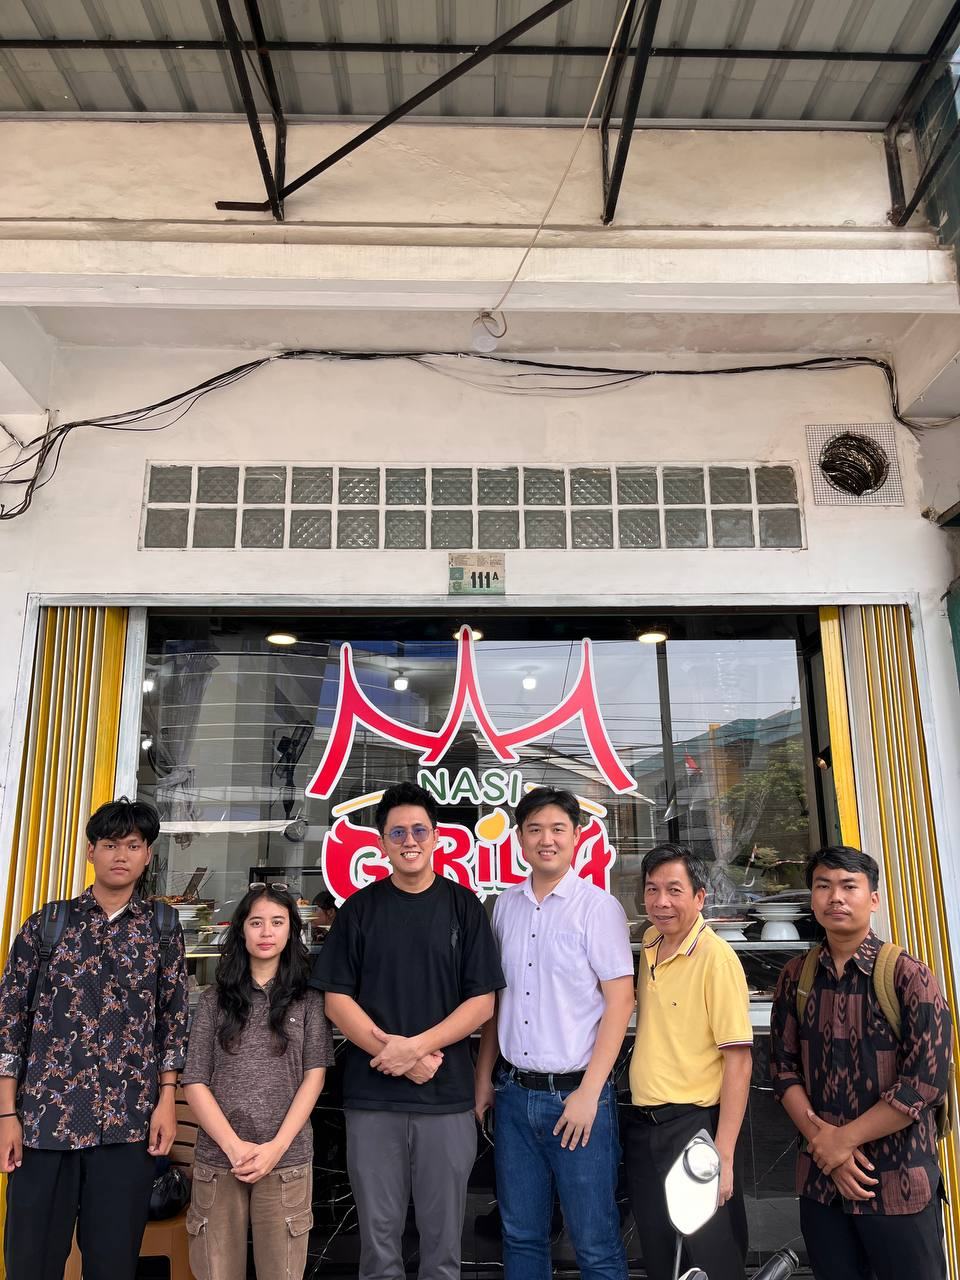
\includegraphics[width=0.78\textwidth,height=0.62\textheight,keepaspectratio]{resource/05-fieldwork/01-wawancara/20260706-wawancara-pemilik/raw/photos/W-PM-20260706-pemilik-nasi-gerilya/W-PM-20260706-foto-01-dokumentasi-bersama-pemilik.jpg}
    \figuresource[0.88\textwidth]{Dokumentasi lapangan bersama pemilik Nasi Gerilya; diolah peneliti (2026).}
    \caption{Dokumentasi Bersama Pemilik Nasi Gerilya}
    \label{fig:dokumentasi-pemilik-nasi-gerilya}
\end{figure}

\FloatBarrier

\begingroup
\scriptsize
\begin{xltabular}{\textwidth}{|C{0.7cm}|L{3.1cm}|Y|}
\caption{Rekap Pokok Temuan Wawancara Kompetitor}
\label{tab:rekap-wawancara-kompetitor} \\
\toprule
\textbf{No.} & \textbf{Informan} & \textbf{Pokok Temuan} \\ \hline
\midrule
\endfirsthead

\continuedtabletitle{3}
\toprule
\textbf{No.} & \textbf{Informan} & \textbf{Pokok Temuan} \\ \hline
\midrule
\endhead

\continuedtablefooter{3}
\endfoot

\bottomrule
\endlastfoot

1 & Kasir Rumah Makan Istana Krakatau & Penjualan masih didominasi pembelian langsung sekitar 80\%. Jam ramai berada pada pukul 11.30--14.00 dan 18.00--19.00. Menu online yang disebut adalah ikan sambal dengan harga sekitar Rp37 ribuan. Promo GrabFood digunakan, namun nilai voucher tidak selalu besar. Keluhan yang muncul adalah pesanan kurang lengkap, item tertinggal, dan driver menunggu. Pengecekan pesanan dilakukan langsung oleh petugas yang mem-packing. Keunggulan usaha terletak pada rasa, pelayanan cepat, porsi online, serta variasi sambal. \\ \hline
2 & Ken, Pondok Krakatau & GrabFood berkontribusi sekitar separuh pesanan. Jam ramai terjadi pada makan siang dan akhir pekan. Menu yang sering dipesan adalah ayam goreng, nasi ayam rendang, nasi ikan kakap, dan nasi ikan nila dengan harga sekitar Rp38 ribuan. Promo tersedia dari platform dan toko. Pelanggan kembali karena rasa enak dan pelayanan cepat. Kendala yang muncul meliputi stok yang belum diperbarui, porsi/rasa yang belum selalu konsisten, driver menunggu, dan item pesanan tertinggal. Pengecekan packing dilakukan melalui jumlah item, kuah, dan kelengkapan lain. \\ \hline
\end{xltabular}
\tablesource[\textwidth]{Wawancara kompetitor dengan Istana Krakatau dan Pondok Krakatau; diolah peneliti (2026).}
\endgroup

\begingroup
\scriptsize
\begin{xltabular}{\textwidth}{|C{0.7cm}|L{3.0cm}|Y|}
\caption{Rekap Pokok Temuan Wawancara Pegawai Nasi Gerilya}
\label{tab:rekap-wawancara-pegawai-nasi-gerilya} \\
\toprule
\textbf{No.} & \textbf{Informan} & \textbf{Pokok Temuan} \\ \hline
\midrule
\endfirsthead

\continuedtabletitle{3}
\toprule
\textbf{No.} & \textbf{Informan} & \textbf{Pokok Temuan} \\ \hline
\midrule
\endhead

\continuedtablefooter{3}
\endfoot

\bottomrule
\endlastfoot

1 & Bella / Laudia Sintiabula Sinalaki & Dapur memiliki pembagian kerja antara leader, senter, butcher, cook, dan helper. Proses kerja dimulai dari pengecekan stok, pengeluaran bahan, pemanasan lauk, dan pengolahan menu utama. Standar resep, takaran, laporan penjualan, dan pengecekan rasa digunakan untuk menjaga kualitas. Menu yang sering dibuat adalah ayam pop dan dendeng. Rendang membutuhkan waktu 5--6 jam, sedangkan ayam goreng membutuhkan proses marinasi. Catatan khusus seperti pemisahan kuah atau sambal masih dapat dipenuhi, tetapi permintaan masak khusus sulit dilakukan karena sistem masak massal. Kendala yang muncul meliputi pesanan mendadak, kondisi ramai, keterlambatan, komunikasi HT yang tidak selalu jelas, menu habis, serta kebutuhan penguatan SOP dan SDM. \\ \hline
2 & Ririn & Kasir berfokus pada pembayaran, sedangkan checker menangani pesanan takeaway dan online. Pesanan GrabFood masuk melalui notifikasi dan print bill, kemudian salinan pesanan ditempel pada box. Aplikasi ojek online dibuka sekitar 09.45 setelah pembaruan lauk. Menu yang sering dipesan melalui GrabFood meliputi ayam goreng, ayam pop, marlin, dan ikan. Staf merekomendasikan menu best seller kepada pelanggan baru, seperti ayam pop, dendeng, cumi, kikil, kepala ikan, dan cincang. Kendala yang muncul antara lain item berkuah rawan tertinggal, nomor pesanan mirip, driver perlu diberi estimasi tunggu, harga GrabFood dipersepsikan berbeda, promo dapat membuat order meningkat, dan komplain perlu ditangani dengan permintaan maaf atau kompensasi. Foto menu dinilai sudah sesuai, tetapi batas request pelanggan tetap perlu dijaga sesuai SOP. \\ \hline
\end{xltabular}
\tablesource[\textwidth]{Wawancara pegawai Nasi Gerilya; diolah peneliti (2026).}
\endgroup

\begingroup
\scriptsize
\begin{xltabular}{\textwidth}{|C{0.7cm}|L{3.3cm}|Y|}
\caption{Rekap Pokok Temuan Wawancara Pendamping Pengembangan Sistem}
\label{tab:rekap-wawancara-pendamping-sistem} \\
\toprule
\textbf{No.} & \textbf{Informan} & \textbf{Pokok Temuan} \\ \hline
\midrule
\endfirsthead

\continuedtabletitle{3}
\toprule
\textbf{No.} & \textbf{Informan} & \textbf{Pokok Temuan} \\ \hline
\midrule
\endhead

\continuedtablefooter{3}
\endfoot

\bottomrule
\endlastfoot

1 & Intern Business Consultant Nasi Gerilya & Pendampingan berfokus pada sistem antrean, absensi digital, menu digital, dan stamp digital. Masalah utama yang diamati adalah antrean dari jalur dine in, ojek online, dan takeaway yang belum sepenuhnya teratur. GrabFood dinilai berperan besar karena pasar ojek online Nasi Gerilya banyak berasal dari platform tersebut. Target potensial meliputi pekerja, mahasiswa, pelanggan sekitar, pelanggan jam makan siang, dan pelanggan yang terbiasa memakai ojek online. Positioning yang perlu diperkuat adalah nasi Padang Medan yang praktis, cepat, lauknya kuat, cocok untuk makan siang, mengenyangkan, dan tetap enak. Ayam pop dinilai layak menjadi hero menu. Tampilan toko digital sudah cukup baik tetapi masih dapat ditingkatkan. Prioritas perbaikan mengarah pada sistem internal yang lebih efektif, efisien, profesional, dan terdigitalisasi. \\ \hline
\end{xltabular}
\tablesource[\textwidth]{Wawancara pendamping pengembangan sistem Nasi Gerilya; diolah peneliti (2026).}
\endgroup

\FloatBarrier
\subsection*{Rekap Kode Temuan Wawancara}
\label{lamp:rekap-kode-temuan-wawancara}

Rekap berikut memuat kode temuan wawancara lapangan yang digunakan sebagai rujukan ringkas dalam Bab IV. Kode disusun menurut kelompok sumber wawancara agar temuan utama dapat dibaca kembali secara lebih lengkap.

\begingroup
\tiny
\begin{xltabular}{\textwidth}{|C{0.9cm}|L{2.15cm}|Y|L{2.4cm}|L{1.95cm}|}
\caption{Rekap Kode Temuan Wawancara Lapangan}
\label{tab:rekap-kode-temuan-wawancara-lapangan} \\
\toprule
\textbf{Kode} & \textbf{Sumber Data} & \textbf{Pokok Temuan} & \textbf{Tema} & \textbf{Kategori} \\ \hline
\midrule
\endfirsthead

\continuedtabletitle{5}
\toprule
\textbf{Kode} & \textbf{Sumber Data} & \textbf{Pokok Temuan} & \textbf{Tema} & \textbf{Kategori} \\ \hline
\midrule
\endhead

\continuedtablefooter{5}
\endfoot

\bottomrule
\endlastfoot
K01.1 & Wawancara pegawai Nasi Gerilya & Dapur memiliki pembagian kerja antara leader, senter, butcher, cook, dan helper. Aktivitas awal mencakup cek stok, mengeluarkan bahan, memanaskan lauk, dan mulai memasak menu utama. & People, process & Kekuatan \\ \hline
K01.2 & Wawancara pegawai Nasi Gerilya & Proses pesanan dari kasir ke dapur dimulai dari konfirmasi pesanan, pengecekan stok, lalu memasak sesuai jenis menu. & Process & Kekuatan \\ \hline
K01.3 & Wawancara pegawai Nasi Gerilya & Jam ramai terutama akhir pekan; pesanan mendadak dan kondisi hectic dapat membuat pesanan menumpuk. & Process & Kelemahan \\ \hline
K01.4 & Wawancara pegawai Nasi Gerilya & Keterlambatan pernah terjadi karena waktu sempit, pesanan mendadak, dan tekanan operasional. & Process, people & Kelemahan \\ \hline
K01.5 & Wawancara pegawai Nasi Gerilya & Dapur menggunakan standar resep, takaran, laporan penjualan, serta double-check rasa dan hasil akhir. & Product, process & Kekuatan \\ \hline
K01.6 & Wawancara pegawai Nasi Gerilya & Menu yang sering dibuat adalah ayam pop dan dendeng; rendang membutuhkan waktu lama dan ayam goreng membutuhkan proses marinasi. & Product & Kelemahan \\ \hline
K01.7 & Wawancara pegawai Nasi Gerilya & Catatan khusus terbatas seperti kuah atau sambal dipisah masih memungkinkan, tetapi permintaan masak khusus sulit dipenuhi karena sistem masak massal. & Product, process & Kelemahan \\ \hline
K01.8 & Wawancara pegawai Nasi Gerilya & Keluhan yang terdengar antara lain aroma kikil, menu habis, dan risiko kualitas bahan tertentu. & Product & Kelemahan \\ \hline
K01.9 & Wawancara pegawai Nasi Gerilya & Komunikasi kasir-dapur memakai HT, tetapi bisa tidak jelas saat area dapur sibuk atau tidak ada yang memegang HT. & People, process & Kelemahan \\ \hline
K01.10 & Wawancara pegawai Nasi Gerilya & Kekuatan utama menurut dapur adalah konsistensi rasa, sedangkan perbaikan utama terkait SOP, SDM, pelayanan floor, dan kecepatan packing. & Product, people, process & Kelemahan \\ \hline
K01.11 & Wawancara pegawai Nasi Gerilya & Kasir berfokus pada pembayaran, sedangkan checker menerima pesanan take away dan pesanan online. & People, process & Kekuatan \\ \hline
K01.12 & Wawancara pegawai Nasi Gerilya & Staf merekomendasikan menu best seller kepada pelanggan baru dan menyesuaikan rekomendasi dengan preferensi pelanggan. & Product, people & Kekuatan \\ \hline
K01.13 & Wawancara pegawai Nasi Gerilya & Aplikasi ojek online dibuka sekitar 09.45; sebelum itu staf wajib memperbarui lauk secara berkala. & Place, process & Kekuatan \\ \hline
K01.14 & Wawancara pegawai Nasi Gerilya & Pesanan GrabFood masuk melalui notifikasi dan print bill; checker menempelkan salinan pesanan pada box. & Process & Kekuatan \\ \hline
K01.15 & Wawancara pegawai Nasi Gerilya & Item basah atau berkuah yang dipisah dari nasi rawan tertinggal, terutama saat kondisi ramai. & Process & Kelemahan \\ \hline
K01.16 & Wawancara pegawai Nasi Gerilya & Nomor GrabFood yang mirip dan driver salah menyebut nomor dapat menyebabkan risiko pesanan tertukar. & Process, place & Kelemahan \\ \hline
K01.17 & Wawancara pegawai Nasi Gerilya & Driver diberi nomor antrean dan staf perlu memberi estimasi tunggu ketika makanan belum selesai. & Process, people & Kelemahan \\ \hline
K01.18 & Wawancara pegawai Nasi Gerilya & Menu yang sering dipesan melalui GrabFood adalah ayam goreng, ayam pop, marlin, dan ikan; kepala ikan cenderung untuk momen tertentu. & Product & Kekuatan \\ \hline
K01.19 & Wawancara pegawai Nasi Gerilya & Harga GrabFood berbeda dari take away dan sesekali dianggap mahal; promo membuat pelanggan membandingkan harga lalu memilih GrabFood. & Price, promotion & Kelemahan \\ \hline
K01.20 & Wawancara pegawai Nasi Gerilya & Promo menyebabkan order membeludak dan harus diinformasikan ke dapur agar stok menu promo siap. & Promotion, process & Kelemahan \\ \hline
K01.21 & Wawancara pegawai Nasi Gerilya & Komplain meliputi porsi ikan, aroma kikil, tingkat pedas, dan makanan yang dianggap bermasalah; respons dilakukan dengan permintaan maaf dan kompensasi. & Product, process, people & Kelemahan \\ \hline
K01.22 & Wawancara pegawai Nasi Gerilya & Foto menu dinilai sudah sesuai dan opsi pesanan cukup banyak, tetapi batas request pelanggan tetap perlu dijaga sesuai SOP. & Physical evidence, product & Kekuatan \\ \hline
K02.1 & Wawancara intern business consultant Nasi Gerilya & Informan adalah mahasiswa magang IT/Sistem Informasi melalui APINDO UMKM Merdeka yang berfokus pada sistem antrean, absensi digital, menu digital, dan stamp digital. & People, process & Kekuatan \\ \hline
K02.2 & Wawancara intern business consultant Nasi Gerilya & Tujuan pendampingan adalah merapikan proses internal agar kerja lebih efektif, efisien, profesional, dan terdigitalisasi. & Process, people & Kekuatan \\ \hline
K02.3 & Wawancara intern business consultant Nasi Gerilya & Keterlibatan informan mencakup observasi kebutuhan operasional, identifikasi kendala lapangan, pembuatan sistem, dan memastikan sistem dapat berjalan. & Process, people & Kekuatan \\ \hline
K02.4 & Wawancara intern business consultant Nasi Gerilya & Data pendampingan berasal dari observasi outlet, jam ramai GrabFood, harga jual GrabFood, pola antrean, kebutuhan karyawan, dan diskusi dengan Nasi Gerilya. & Research input, process & Kekuatan \\ \hline
K02.5 & Wawancara intern business consultant Nasi Gerilya & Masalah utama adalah antrean belum teratur dari tiga jalur; menu digital dan stamp digital dibuat untuk mengurangi beban pencatatan manual dan membangun loyalitas. & Process, promotion, physical evidence & Kelemahan \\ \hline
K02.6 & Wawancara intern business consultant Nasi Gerilya & GrabFood memiliki peran sangat besar karena pasar ojek online terbesar Nasi Gerilya banyak berasal dari GrabFood dan ordernya cukup tinggi. & Place & Peluang \\ \hline
K02.7 & Wawancara intern business consultant Nasi Gerilya & Target potensial adalah pekerja, mahasiswa, pelanggan sekitar, pelanggan jam makan siang, dan pelanggan yang terbiasa memakai ojek online. & STP, place & Peluang \\ \hline
K02.8 & Wawancara intern business consultant Nasi Gerilya & Positioning yang perlu diperkuat adalah nasi Padang Medan yang praktis, cepat, lauknya kuat, cocok untuk makan siang, mengenyangkan, dan tetap enak. & Positioning, product & Kekuatan \\ \hline
K02.9 & Wawancara intern business consultant Nasi Gerilya & Ayam pop dinilai layak menjadi hero menu untuk menarik perhatian pelanggan online. & Product, positioning & Kekuatan \\ \hline
K02.10 & Wawancara intern business consultant Nasi Gerilya & Harga dan promo GrabFood dinilai cukup baik, tetapi diskon atau voucher perlu dihitung agar tidak mengganggu margin, harga jual, dan HPP. & Price, promotion & Kelemahan \\ \hline
K02.11 & Wawancara intern business consultant Nasi Gerilya & Tampilan toko digital sudah cukup baik tetapi masih dapat ditingkatkan; menu digital membuat pengalaman pelanggan lebih praktis dan modern. & Physical evidence, process & Peluang \\ \hline
K02.12 & Wawancara intern business consultant Nasi Gerilya & Promosi penting untuk mendukung sistem digital, terutama agar pelanggan mengetahui menu digital, stamp digital, dan program loyalitas. & Promotion, loyalty & Peluang \\ \hline
K02.13 & Wawancara intern business consultant Nasi Gerilya & Kompetitor relevan menurut informan adalah Pondok Gurih karena sama-sama menyasar pelanggan makanan berat dan lauk khas. & Competition, positioning & Ancaman \\ \hline
K02.14 & Wawancara intern business consultant Nasi Gerilya & Pembeda utama Nasi Gerilya adalah rasa lauk kuat, jumlah pelanggan yang besar, dan kemauan UMKM untuk berbenah melalui sistem digital. & Product, process, differentiation & Kekuatan \\ \hline
K02.15 & Wawancara intern business consultant Nasi Gerilya & Kendala layanan paling berpengaruh terjadi saat makan siang, hari Minggu, dan hari raya ketika pesanan banyak kanal masuk bersamaan dan koordinasi menjadi sulit. & Process, people & Kelemahan \\ \hline
K02.16 & Wawancara intern business consultant Nasi Gerilya & Kelemahan utama adalah pengelolaan data pelanggan dan layanan dine in yang perlu lebih rapi agar usaha tidak hanya bergantung pada platform online. & Promotion, process, loyalty & Kelemahan \\ \hline
K02.17 & Wawancara intern business consultant Nasi Gerilya & Peluang berasal dari kebutuhan makanan cepat, praktis, dan mengenyangkan; ancaman berasal dari persaingan kuliner, biaya platform, kenaikan bahan baku, ekonomi tidak stabil, dan sensitivitas harga. & Opportunity/threat, price & Ancaman \\ \hline
K02.18 & Wawancara intern business consultant Nasi Gerilya & Indikator evaluasi yang relevan adalah jumlah pesanan, omzet, waktu pelayanan, antrean tertangani, repeat order, rating, jumlah komplain, dan efektivitas sistem. & Control, performance & Rekomendasi \\ \hline
K02.19 & Wawancara intern business consultant Nasi Gerilya & Prioritas strategi adalah membuat sistem internal lebih rapi, efektif, efisien, dan profesional melalui sistem antrean, menu digital, stamp digital, dan absensi. & Process, people & Rekomendasi \\ \hline
K02.20 & Wawancara intern business consultant Nasi Gerilya & Rekomendasi terkuat adalah sistem antrean karena masalahnya terlihat langsung; menu digital dan stamp digital relevan tetapi perlu diuji bertahap. & Process, physical evidence, loyalty & Rekomendasi \\ \hline
K02.21 & Wawancara intern business consultant Nasi Gerilya & Strategi Nasi Gerilya tidak hanya soal promosi atau GrabFood; internal yang rapi akan membuat layanan lebih cepat, pelanggan nyaman, dan pemasaran lebih berdampak pada penjualan. & Process, strategy & Rekomendasi \\ \hline
K09.1 & Wawancara pemilik Nasi Gerilya & Komposisi pembelian diperkirakan GrabFood sekitar 50\%, GoFood 12\%, ShopeeFood 8\%, dan offline 30\%. & Place, channel mix & Kekuatan \\ \hline
K09.2 & Wawancara pemilik Nasi Gerilya & Pemasok berasal dari jaringan yang biasa mengirim ke supermarket; bumbu dan sayur dipilih langsung serta dikirim dengan cold storage. & Product, supplier quality & Kekuatan \\ \hline
K09.3 & Wawancara pemilik Nasi Gerilya & Penyimpanan bahan menggunakan freezer peti dan lemari chiller untuk sayur. & Product, process & Kekuatan \\ \hline
K09.4 & Wawancara pemilik Nasi Gerilya & Konsistensi rasa dijaga ketat; pemilik pernah membuang batch rendang ketika urutan masuk rempah membuat rasa berubah. & Product, quality control & Kekuatan \\ \hline
K09.5 & Wawancara pemilik Nasi Gerilya & Margin tidak dibuka karena rahasia; keuntungan belum cukup untuk BEP dan rencana dapur central serta cabang Medan membutuhkan peningkatan keuntungan. & Price, finance & Kelemahan \\ \hline
K09.6 & Wawancara pemilik Nasi Gerilya & Dapur dan frontline memiliki leader masing-masing; leader frontline mengelola GrabFood dan data dikirim ke admin di unit Sambal Gerilya. & People, process & Kekuatan \\ \hline
K09.7 & Wawancara pemilik Nasi Gerilya & Pemasaran melalui KOL makanan pernah dicoba dengan hasil bervariasi tetapi secara keseluruhan membantu penjualan. & Promotion & Peluang \\ \hline
K09.8 & Wawancara pemilik Nasi Gerilya & Kerja sama APINDO menghadirkan mahasiswa magang sebagai business consultant untuk brainstorming pemasaran dan pengembangan usaha. & People, promotion & Peluang \\ \hline
K09.9 & Wawancara pemilik Nasi Gerilya & Toko berstatus halal, meraih Rising Star GrabFood 2025 dan 2026, serta disebut sebagai restoran bintang lima di GrabFood. & Physical evidence, reputation & Kekuatan \\ \hline
K09.10 & Wawancara pemilik Nasi Gerilya & Usaha sedang mengembangkan Flowie untuk mengecek stok dan HPP di toko. & Process, technology & Kekuatan \\ \hline
K09.11 & Wawancara pemilik Nasi Gerilya & Leader diajarkan independen agar dapat bekerja tanpa campur tangan langsung pemilik. & People & Kekuatan \\ \hline
K09.12 & Wawancara pemilik Nasi Gerilya & Regenerasi dilakukan dengan mendidik wakil leader. & People & Kekuatan \\ \hline
K03.1 & Wawancara kompetitor & GrabFood menyumbang sekitar lebih kurang 50 persen dari total pesanan Pondok Krakatau. & Place & Ancaman \\ \hline
K03.2 & Wawancara kompetitor & Jam ramai Pondok Krakatau berada pada makan siang dan akhir pekan. & Place, process & Ancaman \\ \hline
K03.3 & Wawancara kompetitor & Menu sering dipesan di Pondok Krakatau adalah ayam goreng, nasi ayam rendang, nasi ikan kakap, dan nasi ikan nila dengan harga sekitar Rp38 ribuan. & Product, price & Ancaman \\ \hline
K03.4 & Wawancara kompetitor & Pelanggan kembali karena rasa enak dan pelayanan cepat. & Product, people, process & Ancaman \\ \hline
K03.5 & Wawancara kompetitor & Promo tersedia dari GrabFood dan kadang dibuat oleh toko. & Promotion, price & Ancaman \\ \hline
K03.6 & Wawancara kompetitor & Stok habis kadang belum diperbarui di platform ketika pelanggan sudah order. & Process, place & Peluang \\ \hline
K03.7 & Wawancara kompetitor & Porsi dan rasa kadang tidak konsisten karena petugas bungkus atau masak berbeda. & Product, people & Peluang \\ \hline
K03.8 & Wawancara kompetitor & Pesanan kadang tertinggal, lalu dikirim ulang melalui Grab untuk disusulkan. & Process & Peluang \\ \hline
K03.9 & Wawancara kompetitor & Pengecekan packing dilakukan melalui jumlah item, kuah, dan kelengkapan lain. & Process & Ancaman \\ \hline
K03.10 & Wawancara kompetitor & Penjualan Istana Krakatau masih didominasi offline sekitar 80 persen. & Place & Ancaman \\ \hline
K03.11 & Wawancara kompetitor & Jam ramai Istana Krakatau terjadi pada 11.30--14.00 dan sekitar 18.00--19.00. & Place, process & Ancaman \\ \hline
K03.12 & Wawancara kompetitor & Menu online yang disebut adalah ikan sambal dengan harga sekitar Rp37 ribuan. & Product, price & Ancaman \\ \hline
K03.13 & Wawancara kompetitor & Pelanggan memilih Istana Krakatau karena rasa dan pelayanan cepat. & Product, process & Ancaman \\ \hline
K03.14 & Wawancara kompetitor & Promo sering dipakai terutama di GrabFood, walaupun voucher disebut tidak besar. & Promotion & Ancaman \\ \hline
K03.15 & Wawancara kompetitor & Pesanan kurang lengkap menjadi keluhan pelanggan. & Process & Peluang \\ \hline
K03.16 & Wawancara kompetitor & Pesanan tertinggal membuat driver lama menunggu. & Process & Peluang \\ \hline
K03.17 & Wawancara kompetitor & Pengecekan dilakukan langsung oleh petugas yang mem-packing. & Process & Ancaman \\ \hline
K03.18 & Wawancara kompetitor & Keunggulan Istana Krakatau ada pada sambal empat jenis, terutama sambal Padang, serta rasa dan porsi online yang lebih besar. & Product & Ancaman \\ \hline
\end{xltabular}
\tablesource[\textwidth]{Wawancara lapangan 1--4 Juli 2026; diolah peneliti (2026).}
\endgroup

\subsection*{Dokumentasi Wawancara Kompetitor Istana Krakatau}

Dokumentasi berikut memperlihatkan suasana wawancara lapangan dan kondisi pendukung pada Rumah Makan Istana Krakatau. Data ini digunakan sebagai pelengkap catatan wawancara kompetitor dalam membaca layanan, tampilan usaha, dan konteks pembanding GrabFood.

\begin{figure}[!p]
    \centering
    \begin{minipage}[t]{0.48\textwidth}
        \centering
        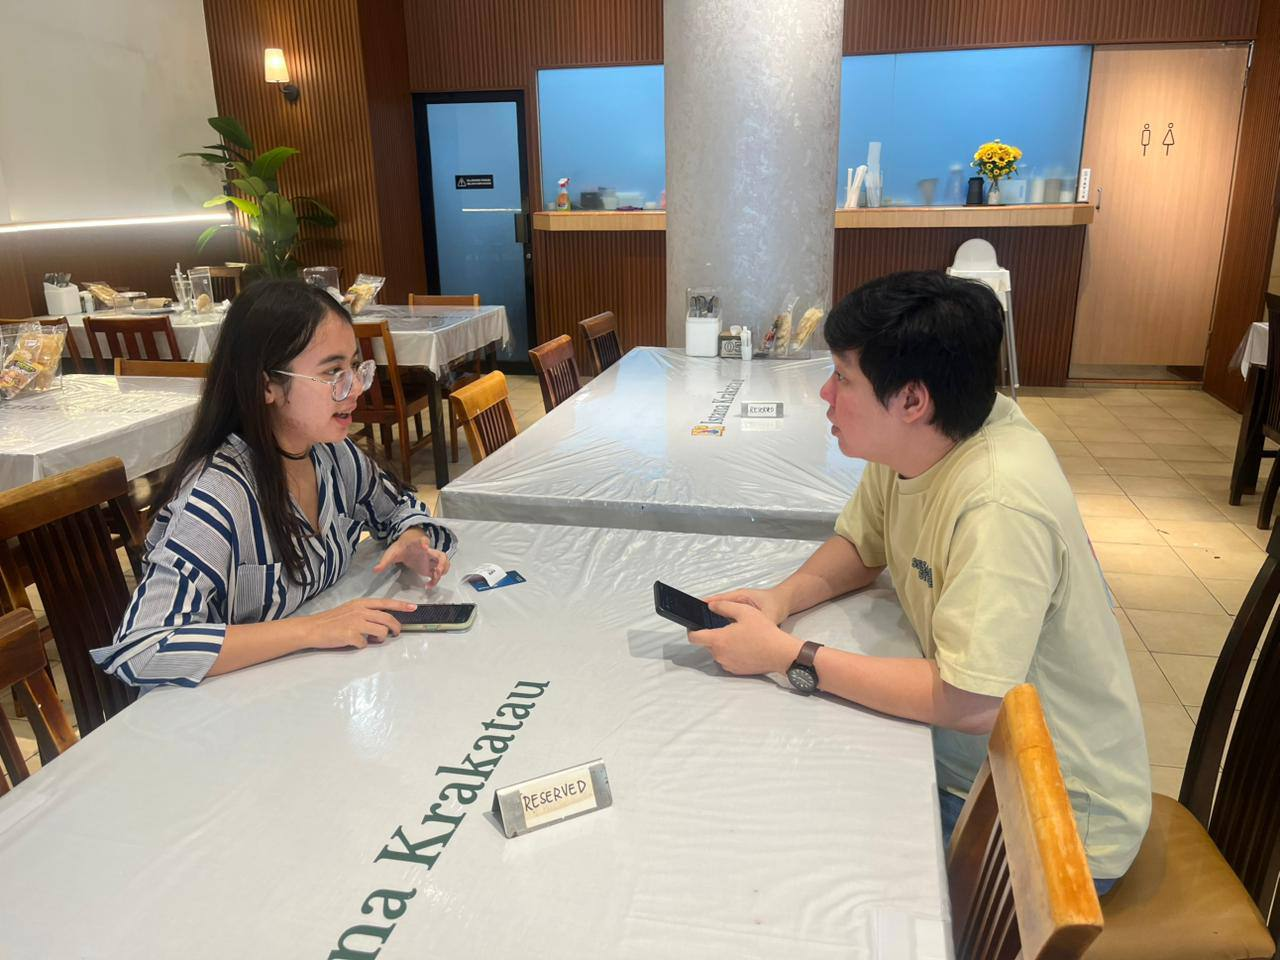
\includegraphics[width=\linewidth,height=0.30\textheight,keepaspectratio]{resource/05-fieldwork/01-wawancara/20260701-20260704-wawancara-lapangan/raw/photos/K03-PB-20260703-istana-krakatau/K03-PB-20260703-foto-01-suasana-wawancara.jpg}
        \par\footnotesize (a) Suasana wawancara kompetitor
    \end{minipage}\hfill
    \begin{minipage}[t]{0.48\textwidth}
        \centering
        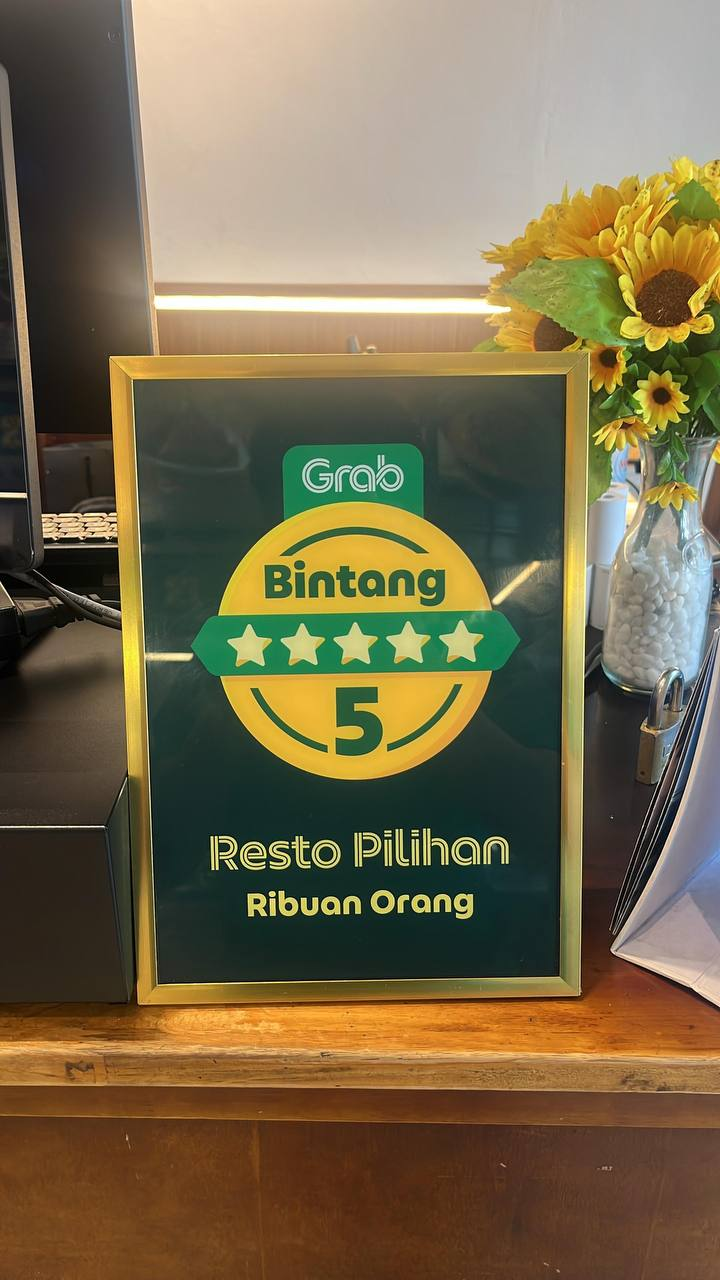
\includegraphics[width=\linewidth,height=0.30\textheight,keepaspectratio]{resource/05-fieldwork/01-wawancara/20260701-20260704-wawancara-lapangan/raw/photos/K03-PB-20260703-istana-krakatau/K03-PB-20260703-foto-02-plakat-grab.jpg}
        \par\footnotesize (b) Atribut reputasi layanan
    \end{minipage}

    \vspace{6pt}

    \begin{minipage}[t]{0.48\textwidth}
        \centering
        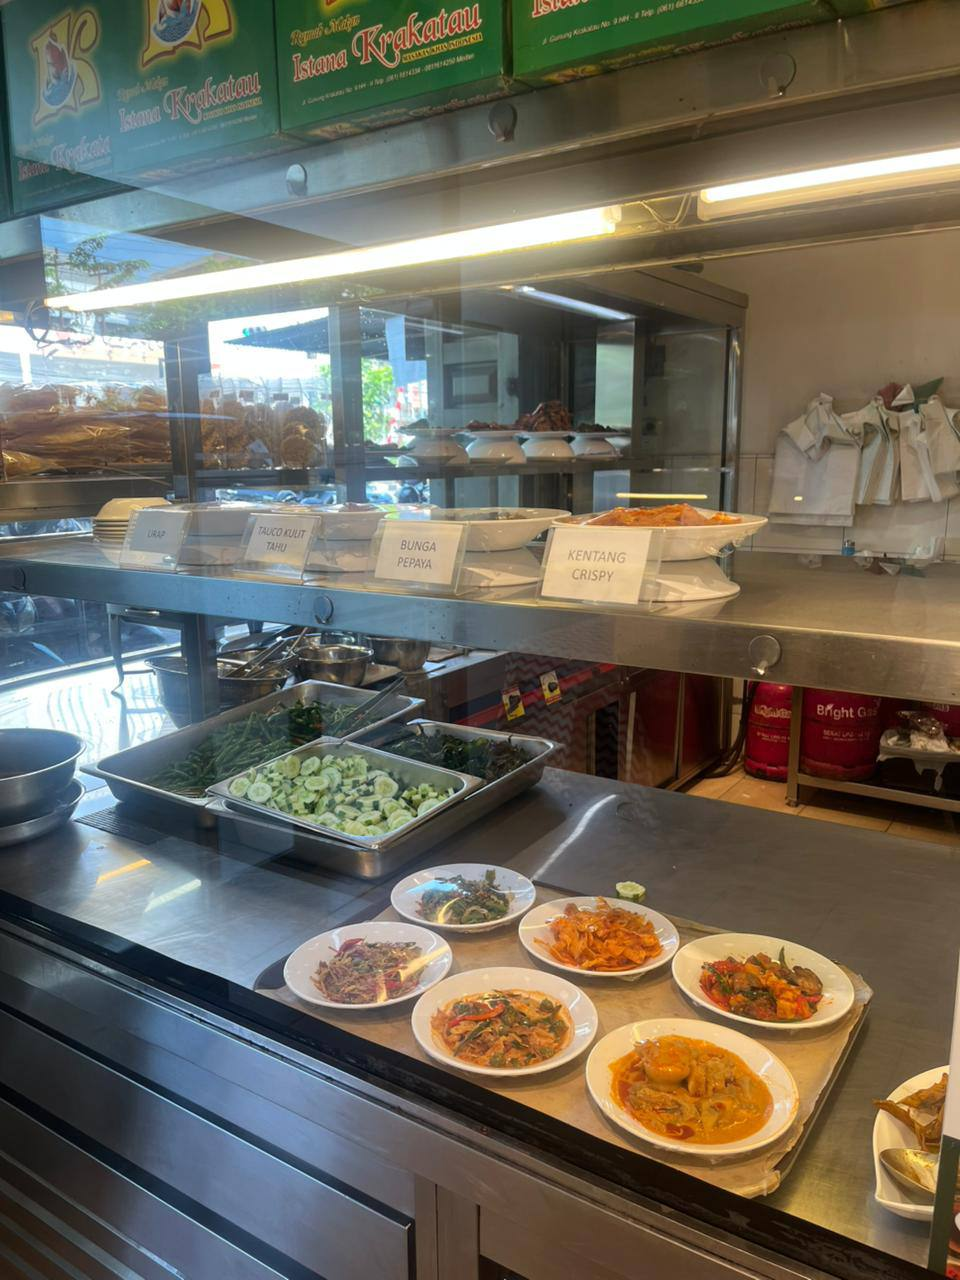
\includegraphics[width=\linewidth,height=0.30\textheight,keepaspectratio]{resource/05-fieldwork/01-wawancara/20260701-20260704-wawancara-lapangan/raw/photos/K03-PB-20260703-istana-krakatau/K03-PB-20260703-foto-03-etalase-lauk.jpg}
        \par\footnotesize (c) Etalase lauk
    \end{minipage}\hfill
    \begin{minipage}[t]{0.48\textwidth}
        \centering
        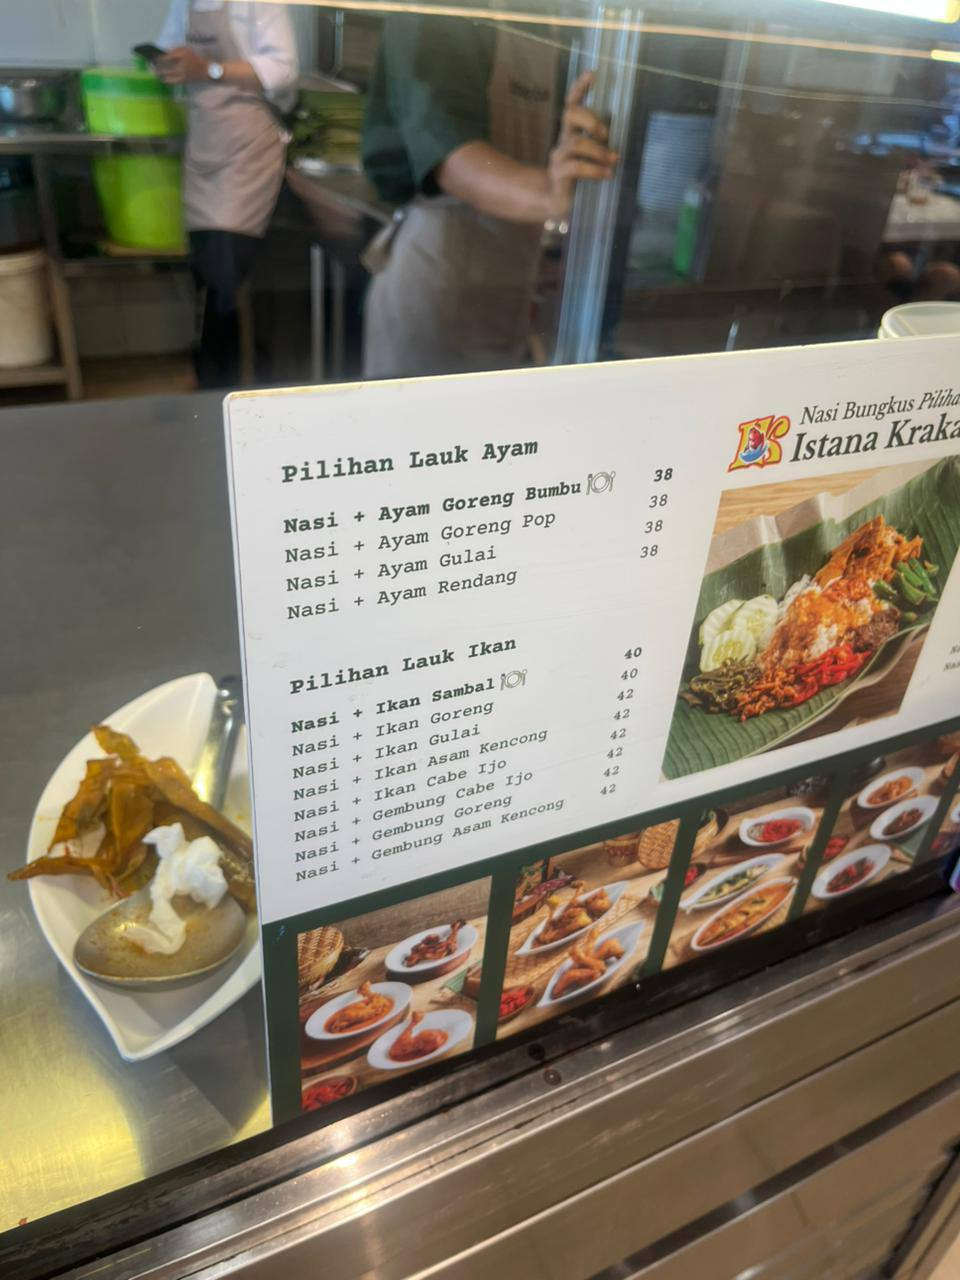
\includegraphics[width=\linewidth,height=0.30\textheight,keepaspectratio]{resource/05-fieldwork/01-wawancara/20260701-20260704-wawancara-lapangan/raw/photos/K03-PB-20260703-istana-krakatau/K03-PB-20260703-foto-04-menu-paket.jpg}
        \par\footnotesize (d) Menu paket
    \end{minipage}
    \figuresource[0.98\textwidth]{Dokumentasi lapangan pada Rumah Makan Istana Krakatau; diolah peneliti (2026).}
    \caption{Dokumentasi Wawancara Kompetitor di Rumah Makan Istana Krakatau}
    \label{fig:dokumentasi-wawancara-istana-krakatau}
\end{figure}

\FloatBarrier
\subsection*{Dokumentasi Wawancara Kompetitor Pondok Krakatau}

Dokumentasi berikut memperlihatkan situasi pengumpulan data lapangan pada Pondok Krakatau, mencakup interaksi dengan narasumber serta konteks menu yang terlihat di lokasi wawancara. Dokumentasi ini digunakan sebagai pelengkap catatan wawancara kompetitor Pondok Krakatau.
\begin{figure}[!hbp]
    \centering
    \setlength{\abovecaptionskip}{4pt}
    \setlength{\belowcaptionskip}{0pt}
    \begin{minipage}[t]{0.47\textwidth}
        \centering
        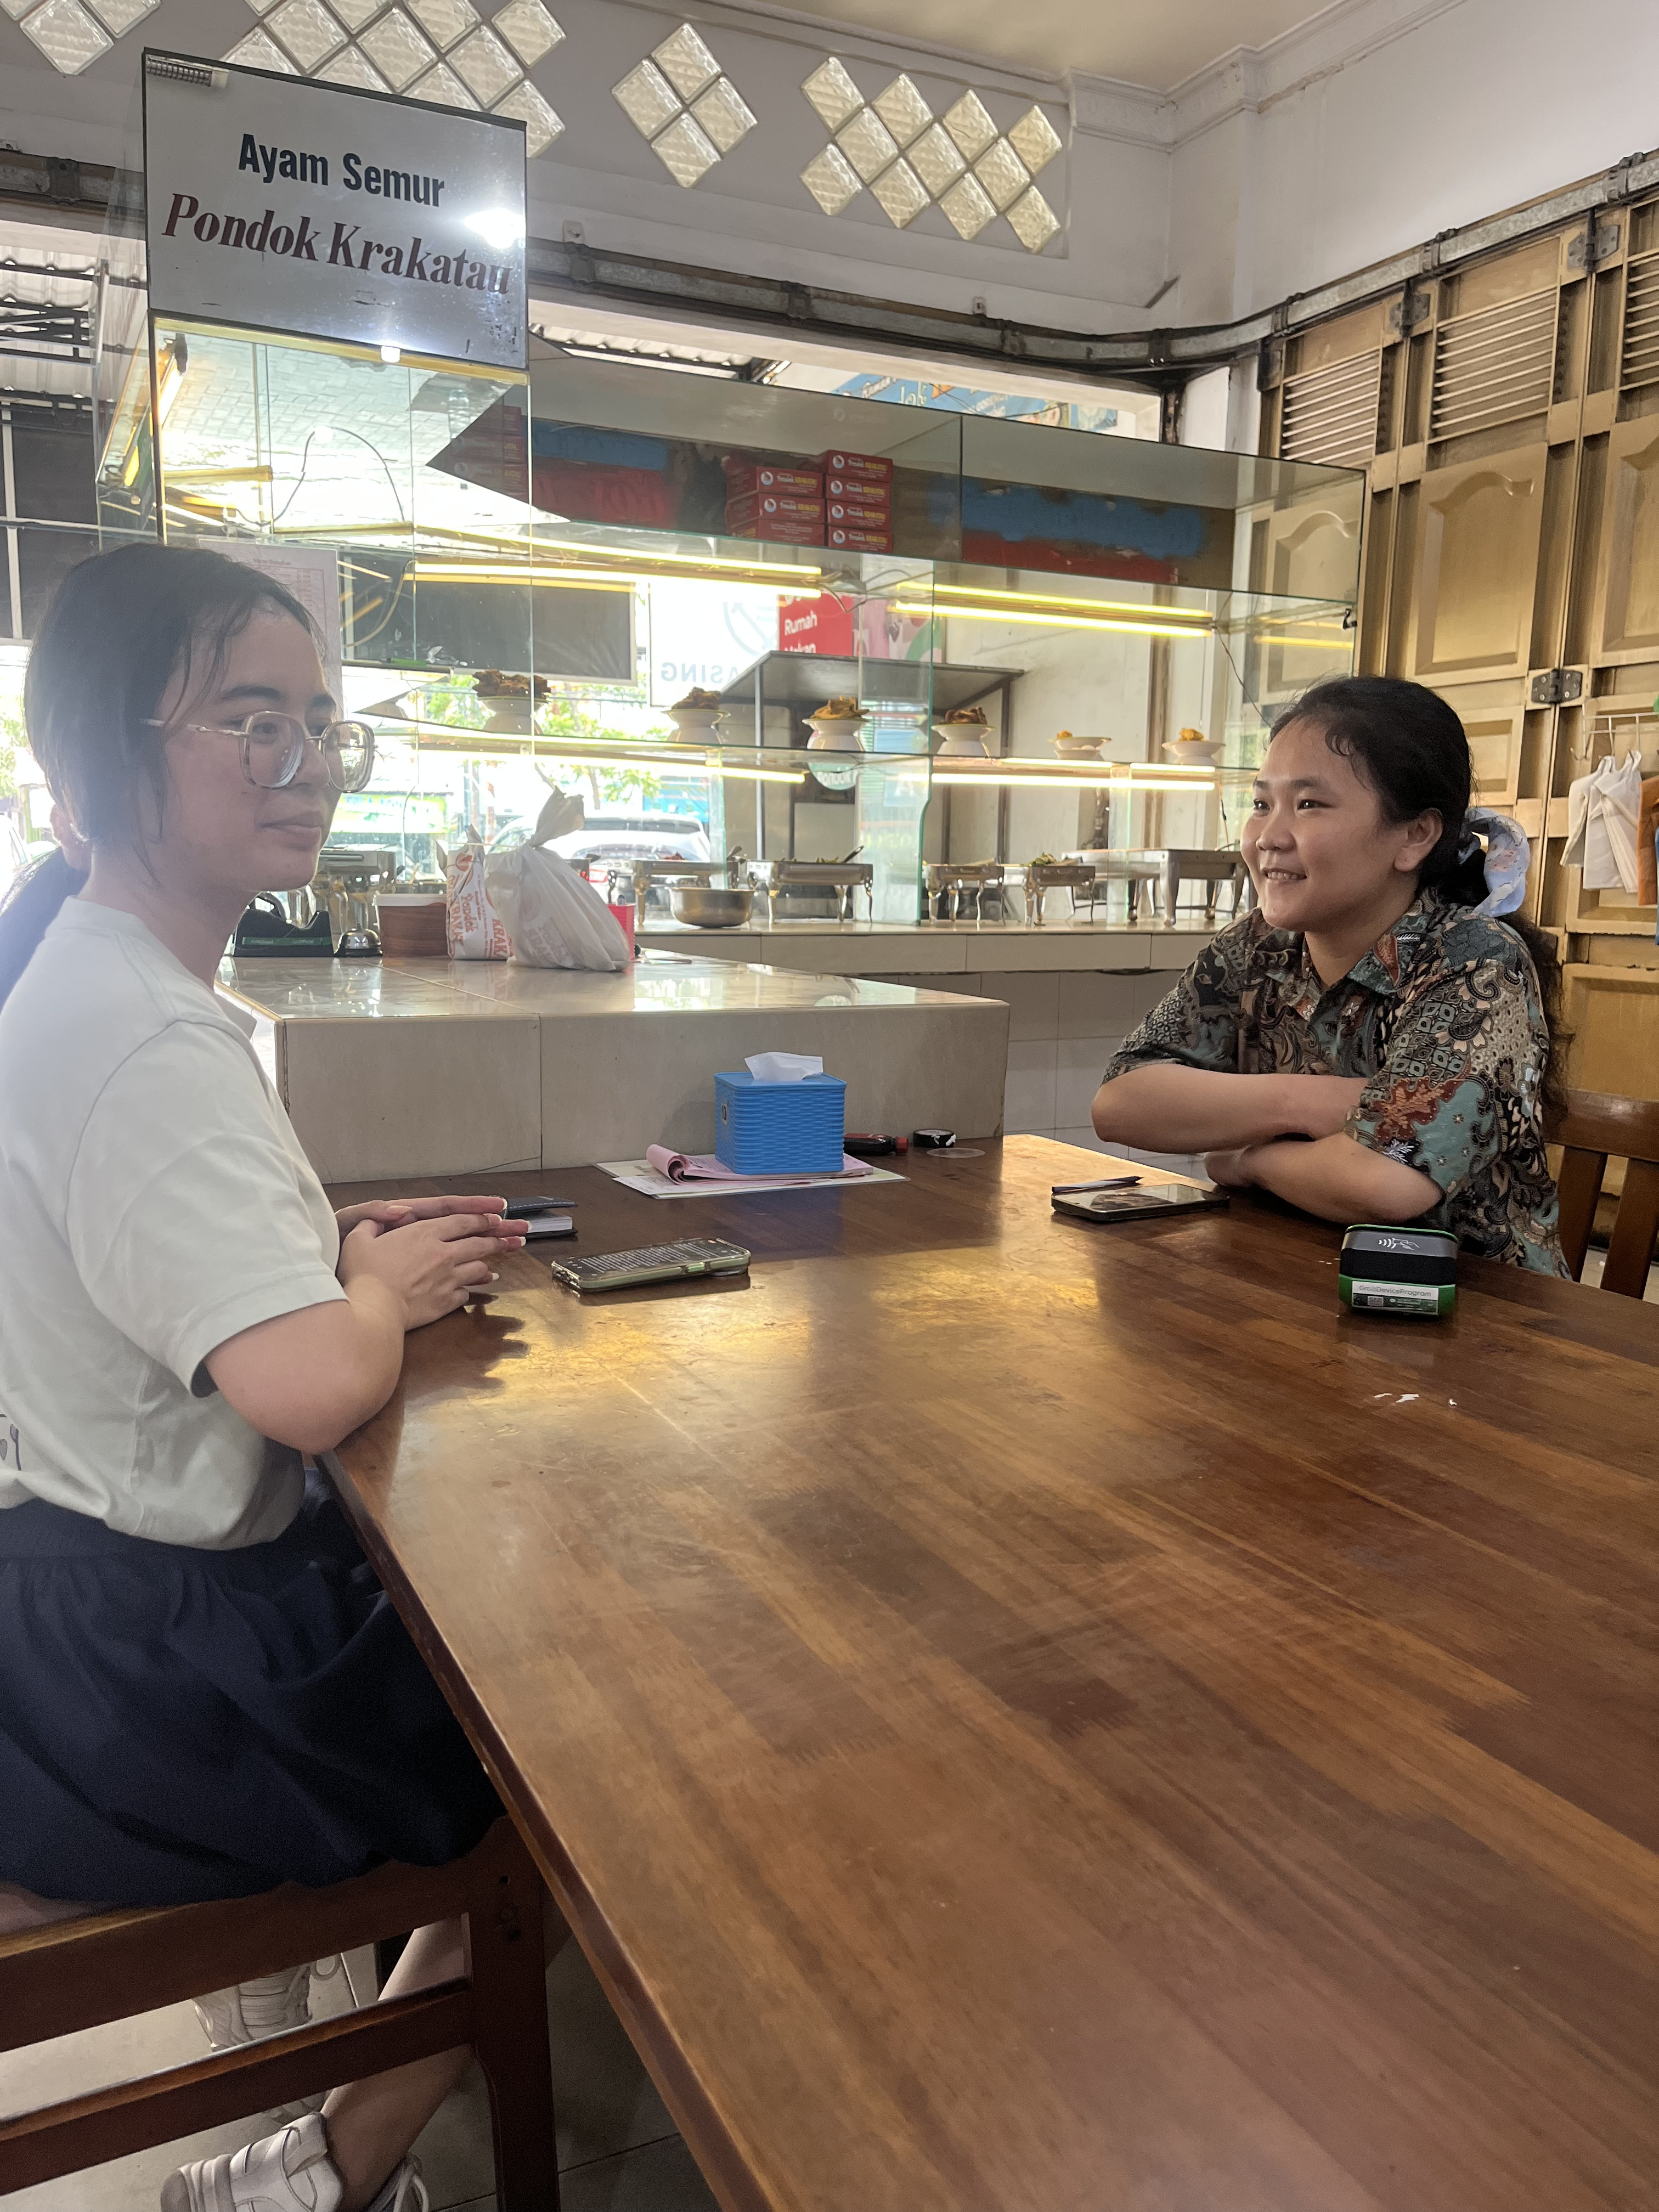
\includegraphics[width=\linewidth,height=0.245\textheight,keepaspectratio]{resource/05-fieldwork/01-wawancara/20260701-20260704-wawancara-lapangan/raw/photos/K03-PA-20260703-pondok-krakatau/K03-PA-20260703-foto-12.jpg}
        \par\vspace{2pt}\footnotesize (a) Dokumentasi kegiatan wawancara dengan narasumber
    \end{minipage}\hfill
    \begin{minipage}[t]{0.47\textwidth}
        \centering
        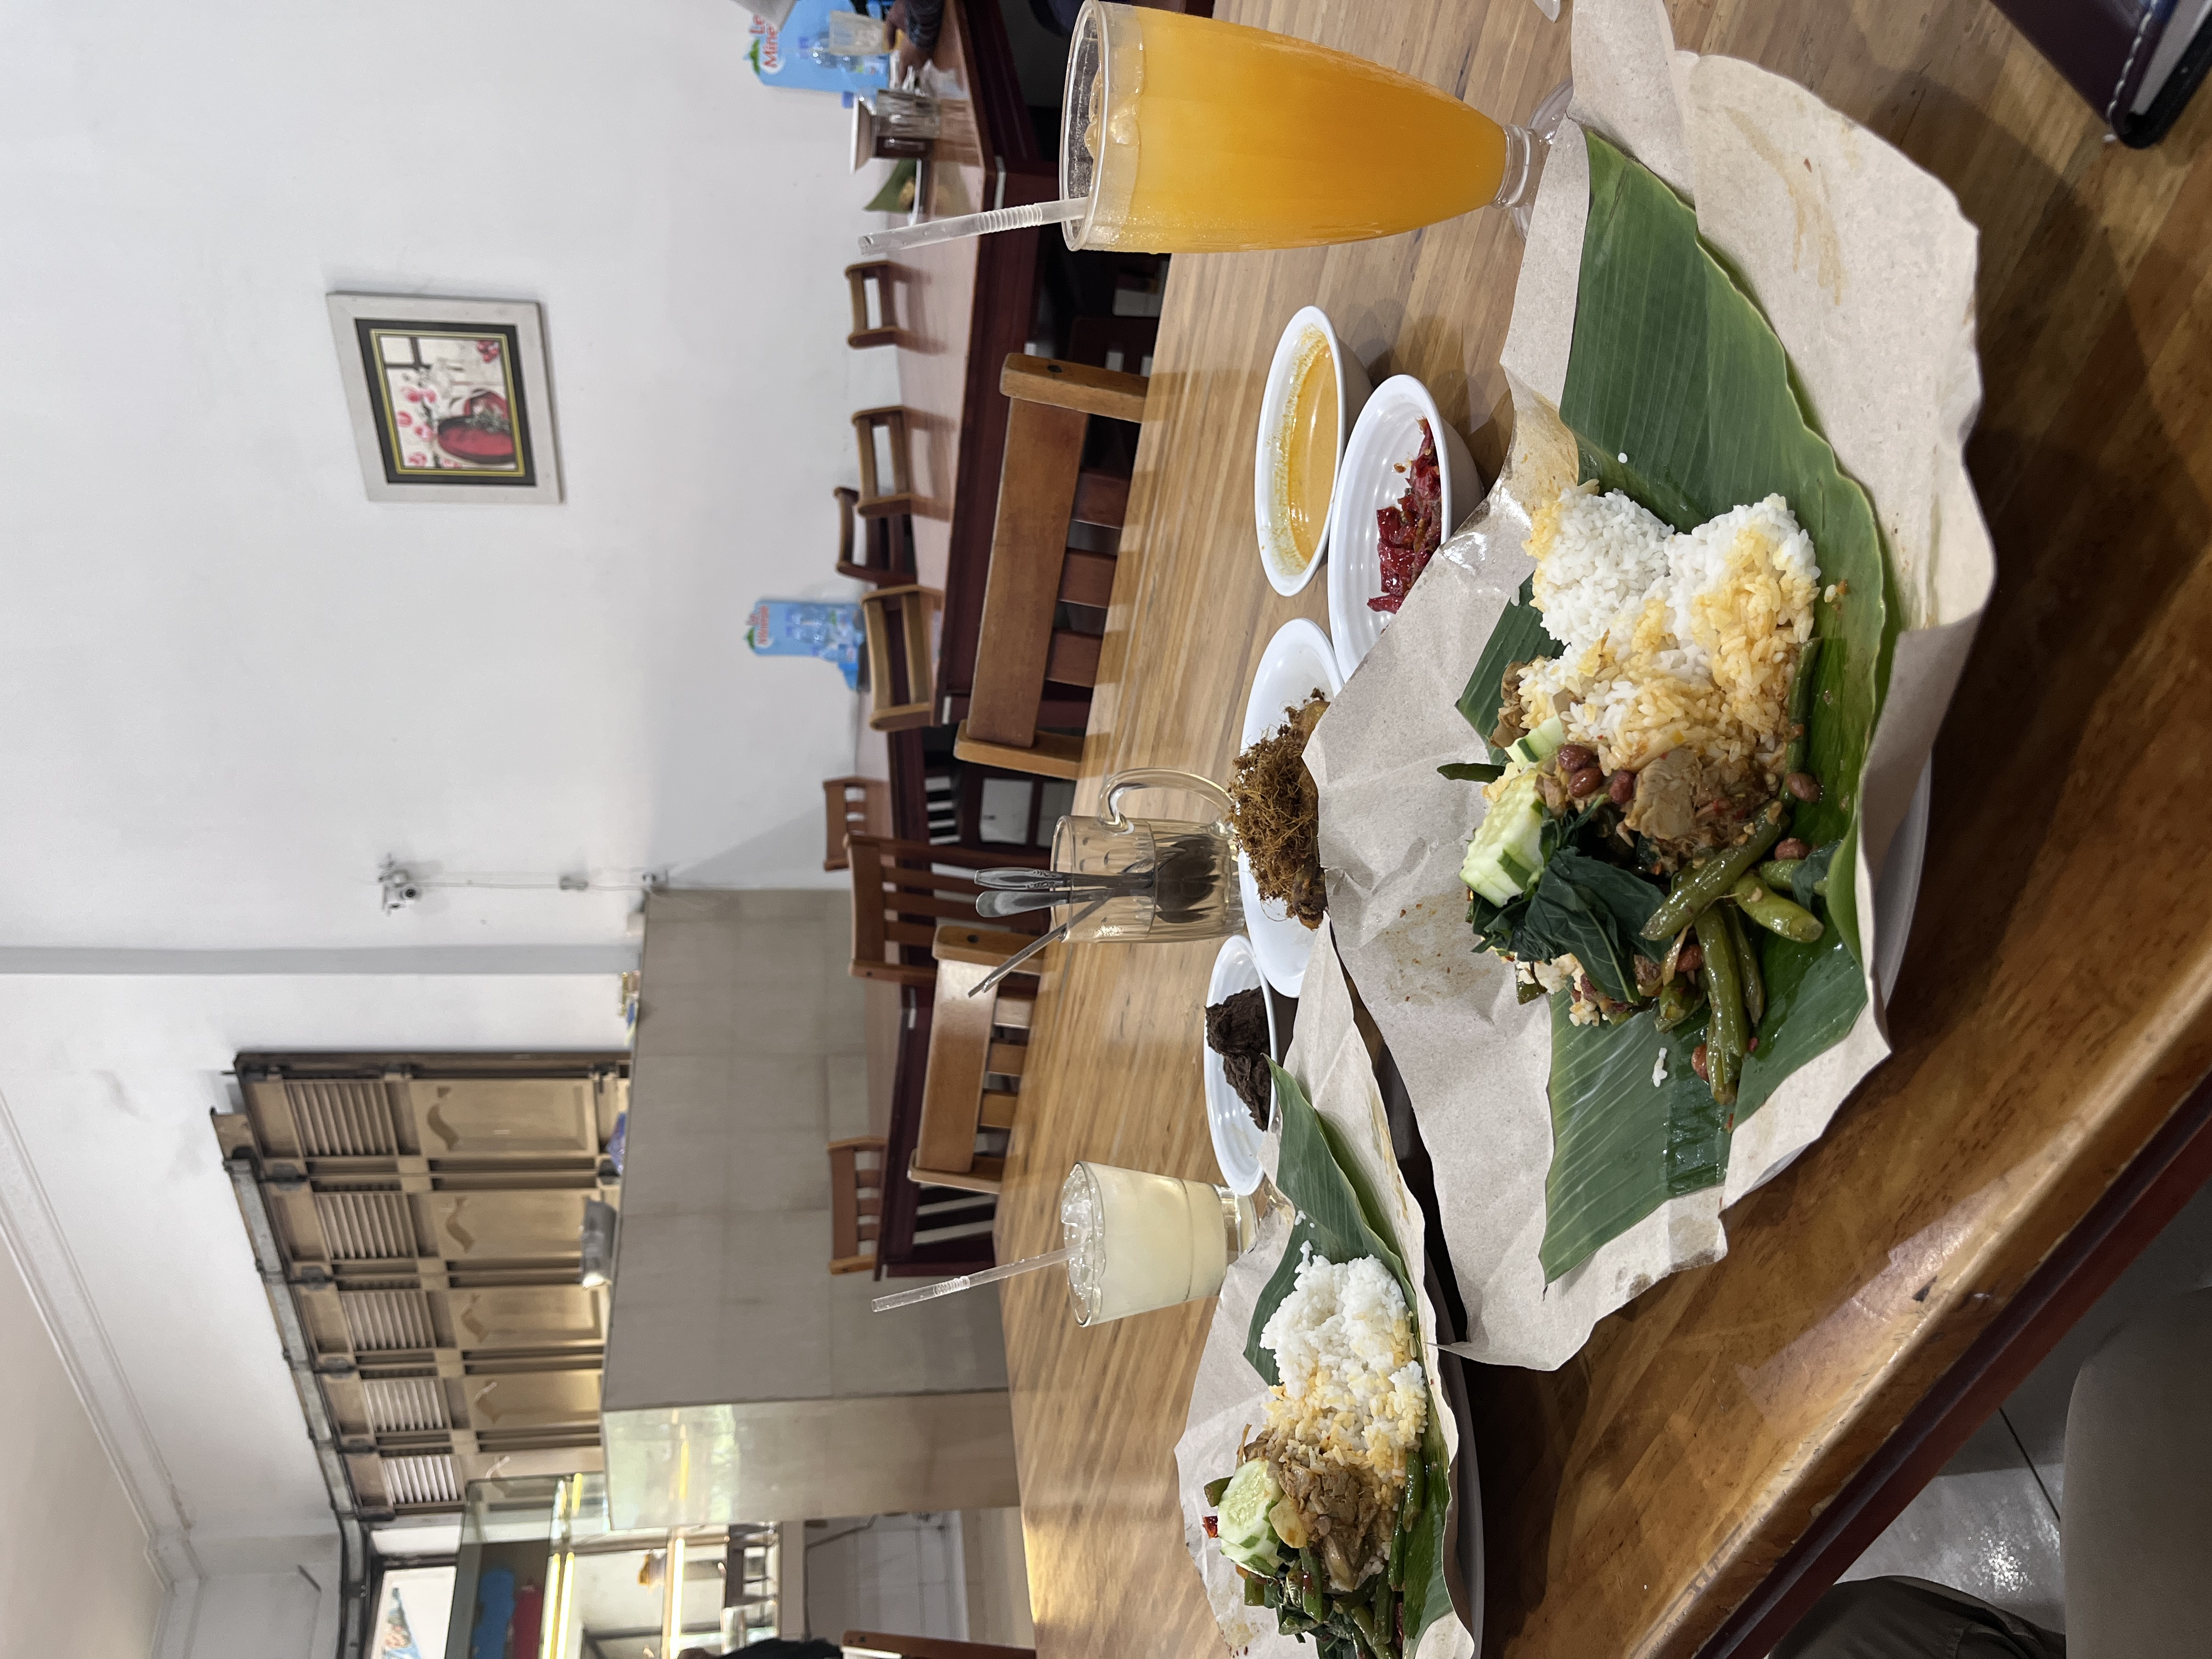
\includegraphics[angle=-90,origin=c,width=\linewidth,height=0.245\textheight,keepaspectratio]{resource/05-fieldwork/01-wawancara/20260701-20260704-wawancara-lapangan/raw/photos/K03-PA-20260703-pondok-krakatau/K03-PA-20260703-foto-07.jpg}
        \par\vspace{2pt}\footnotesize (b) Suasana interaksi di lokasi penelitian
    \end{minipage}

    \vspace{4pt}

    \begin{minipage}[t]{0.47\textwidth}
        \centering
        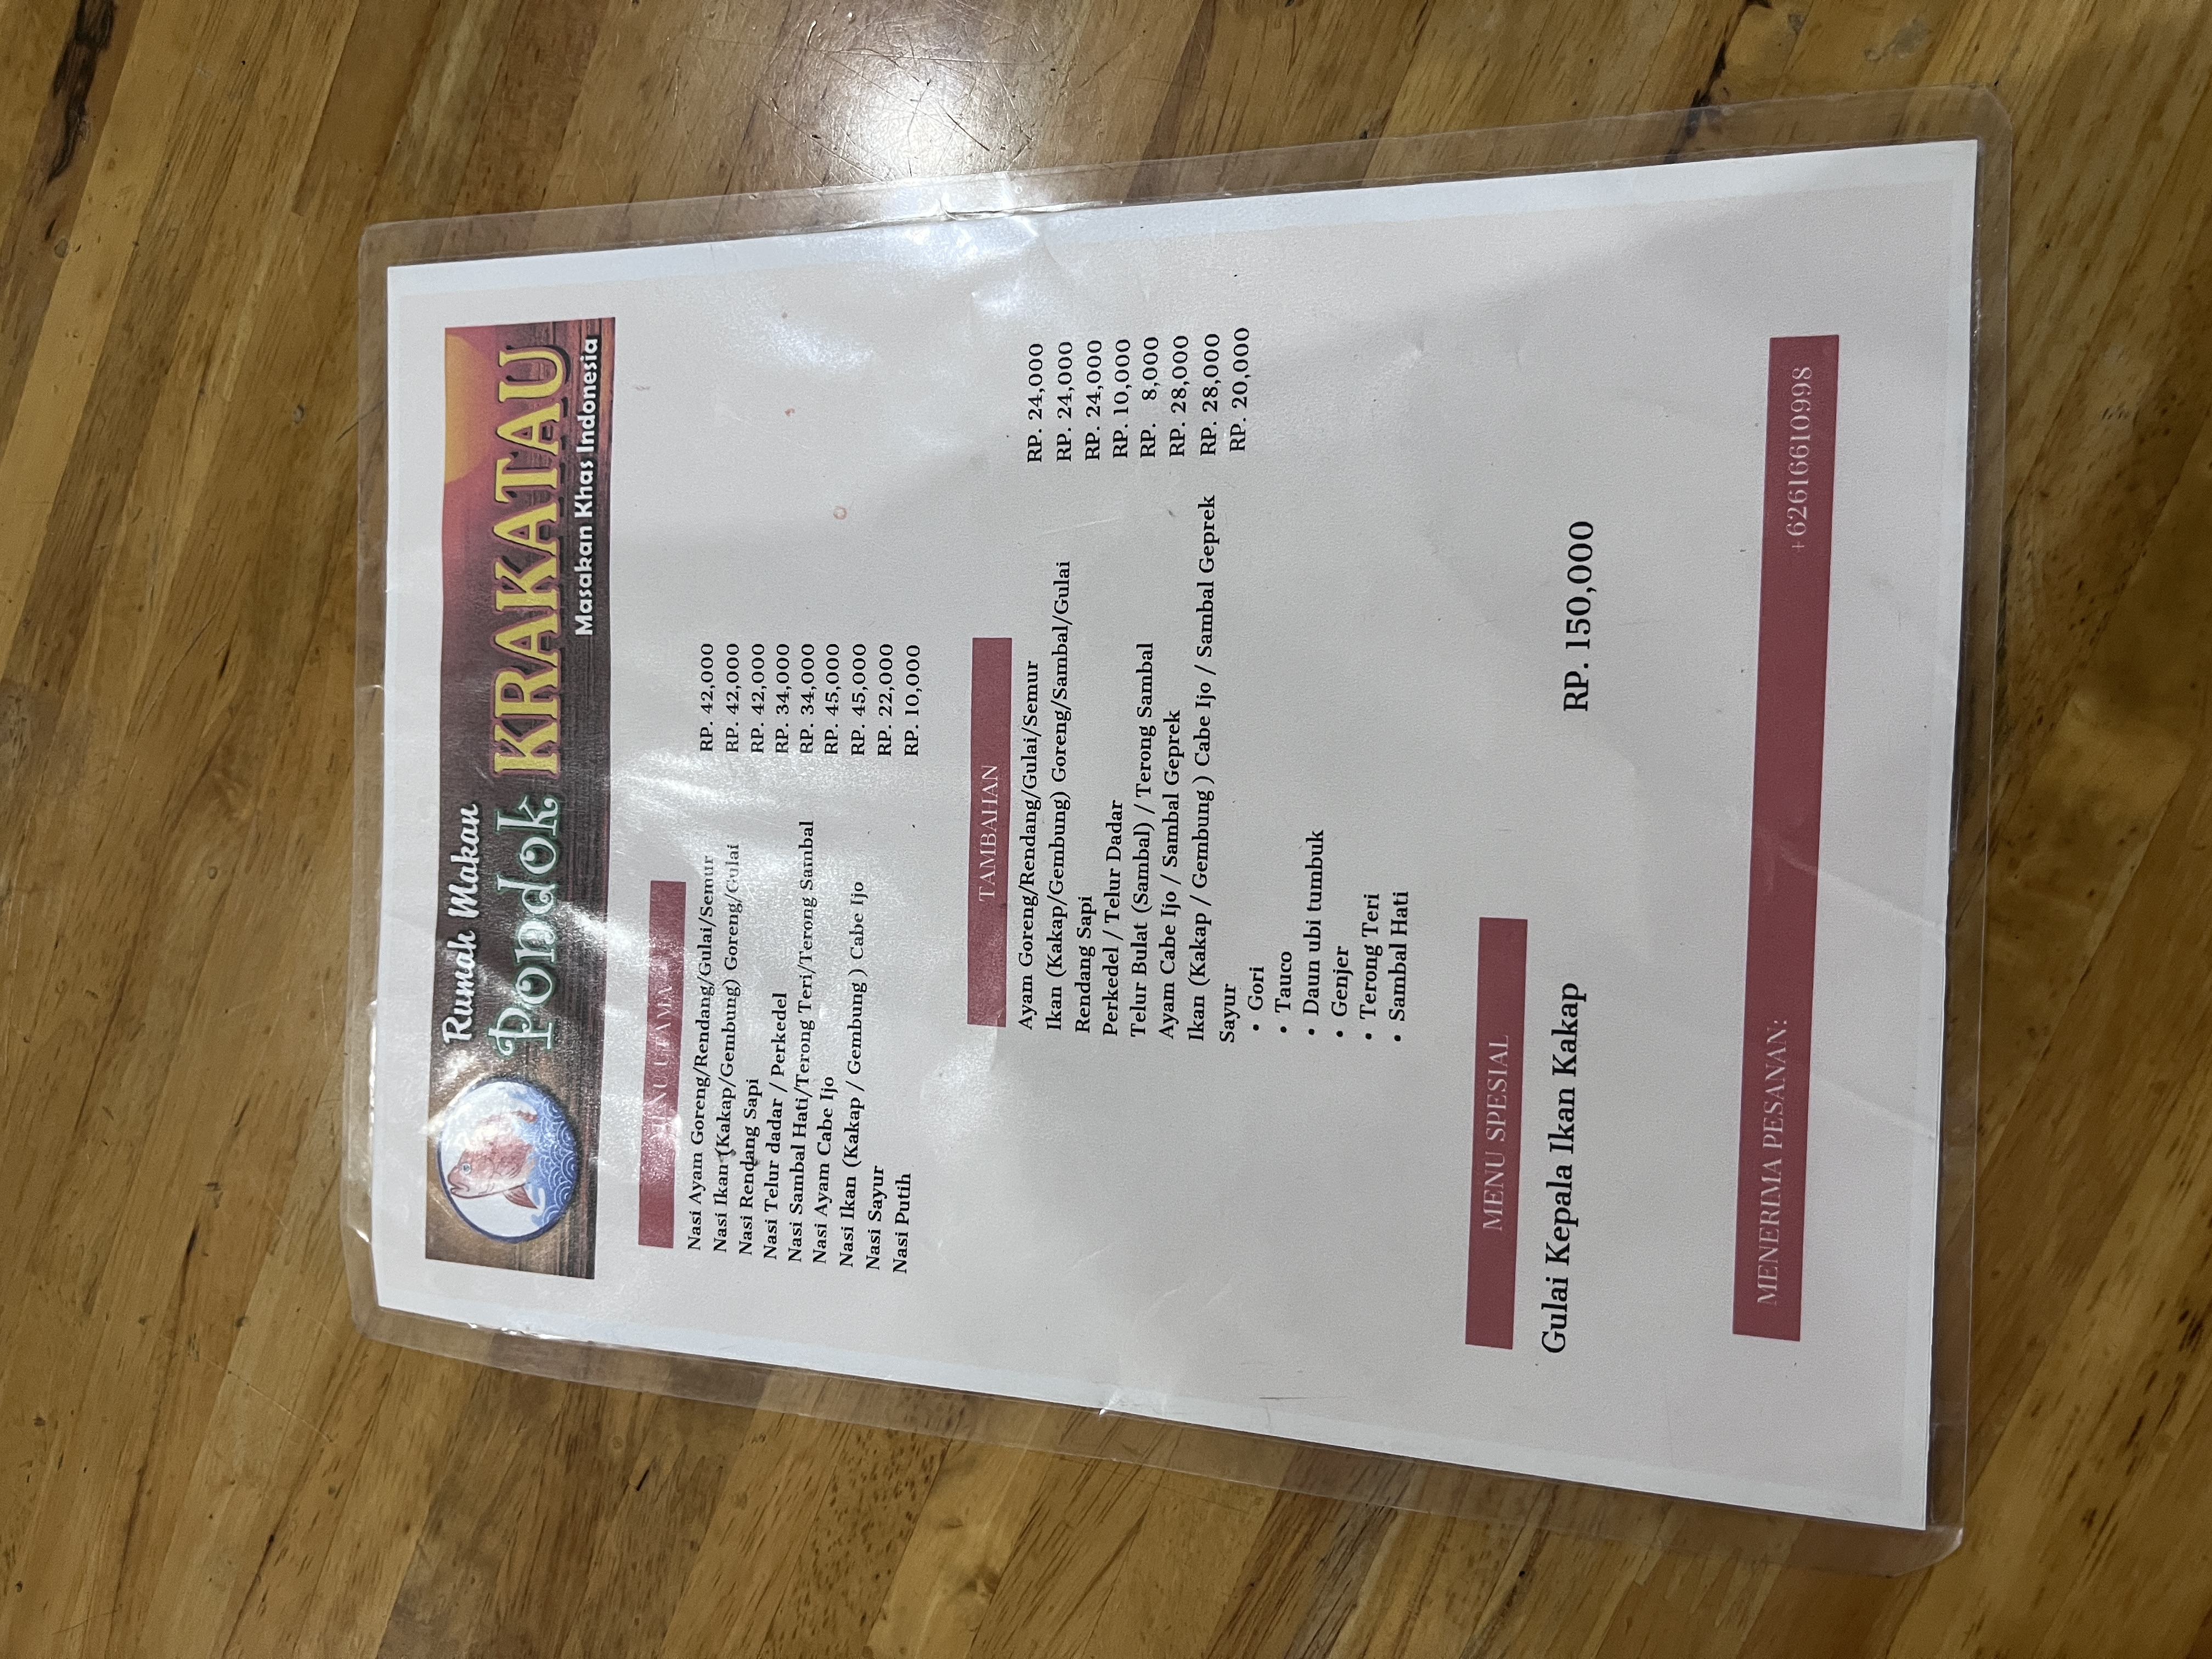
\includegraphics[angle=-90,origin=c,width=\linewidth,height=0.245\textheight,keepaspectratio]{resource/05-fieldwork/01-wawancara/20260701-20260704-wawancara-lapangan/raw/photos/K03-PA-20260703-pondok-krakatau/K03-PA-20260703-foto-01.jpg}
        \par\vspace{2pt}\footnotesize (c) Dokumentasi menu rumah makan
    \end{minipage}\hfill
    \begin{minipage}[t]{0.47\textwidth}
        \centering
        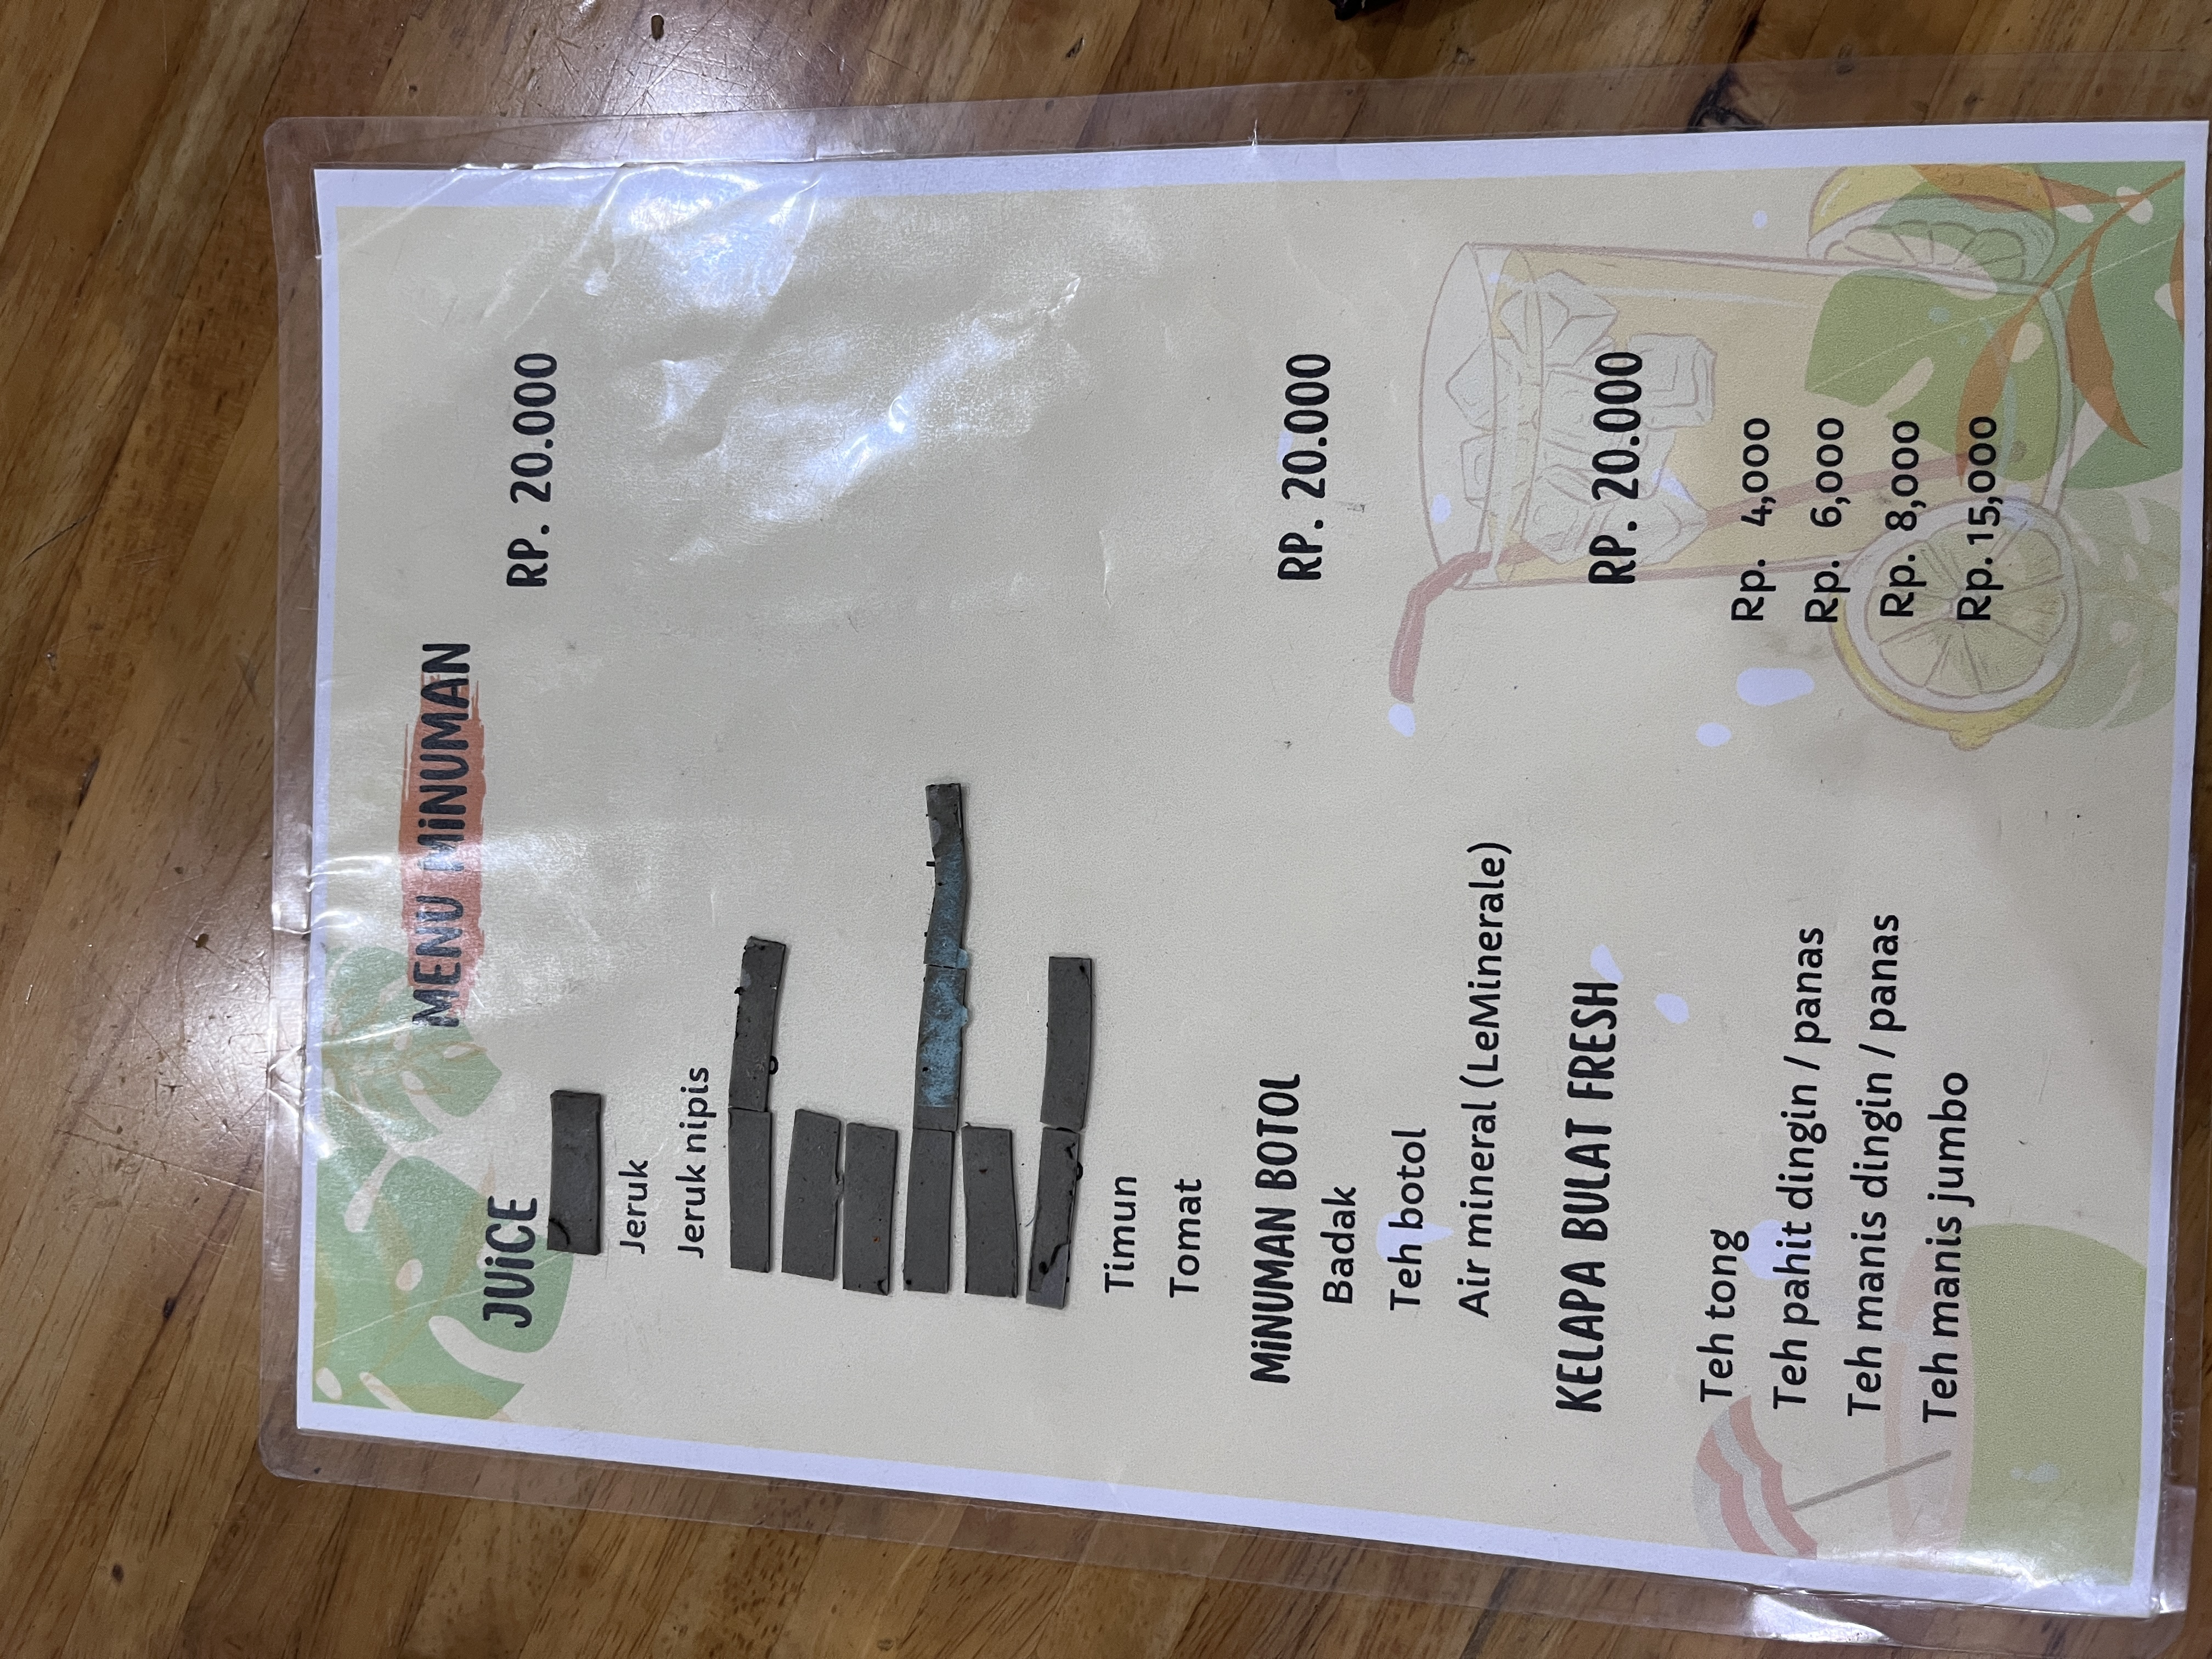
\includegraphics[angle=-90,origin=c,width=\linewidth,height=0.245\textheight,keepaspectratio]{resource/05-fieldwork/01-wawancara/20260701-20260704-wawancara-lapangan/raw/photos/K03-PA-20260703-pondok-krakatau/K03-PA-20260703-foto-02.jpg}
        \par\vspace{2pt}\footnotesize (d) Dokumentasi menu minuman di lokasi
    \end{minipage}
    \figuresource[0.98\textwidth]{Dokumentasi lapangan pada Pondok Krakatau; diolah peneliti (2026).}
    \caption{Dokumentasi Wawancara Kompetitor di Pondok Krakatau}
    \label{fig:dokumentasi-wawancara-pondok-krakatau}
\end{figure}

\FloatBarrier
